In another example in Figure~\ref{fig:abscfg_ifQuery}(a), the answer of a query request is used in the guard of the if control. The
query request, $\clabel{\assign{y}{\query(\chi[2])}}^2$  in the first branch may-depend on
the first query $\clabel{\assign{x}{\query(\chi[1])}}^0$ through the control dependency.
Adaptivity in this graph is $2$, which is correctly be captured by Definition~\ref{def:trace_adapt}.
Its abstract transition graph is generated as in Figure~\ref{fig:abscfg_ifQuery}(b).
The result of the first query request is used in the guard of the if command, the graph
capture this relation through two branches
$1 \xrightarrow{x>2} 2$ and $1 \xrightarrow{x \leq 2} 3$.
Constraints on the two edges are summarized from the guard $\clabel{x > 2}^1$ through Definition~\ref{def:constraint_compute}.
In this sense, the following static analysis based on this graph is able to analyze the dependency relation passing through control flow.
\begin{figure} 
    \centering
    \begin{subfigure}{1.0\textwidth}
      \begin{centering}
      $
          \begin{array}{l}
          \kw{ifQuery} \triangleq \\
          \clabel{\assign{x}{\query(\chi[1])}}^0 ; 
          \eif( \clabel{x > 2}^1 , \clabel{\assign{y}{\query(\chi[2])}}^2, \clabel{\eskip}^3 )
          \end{array}
      $
      \caption{}
      \end{centering}
      \end{subfigure}
    \begin{subfigure}{.47\textwidth}
        \begin{centering}
      \begin{tikzpicture}[scale=\textwidth/20cm,samples=200]
      \draw[] (0, 10) circle (0pt) node{{ $0$}};
      \draw[] (0, 7) circle (0pt) node{{ $1$}};
      \draw[] (-3, 3) circle (0pt) node{\textbf{$2$}};
      \draw[] (3, 3) circle (0pt) node{{ $3$}};
      \draw[] (0, -1) circle (0pt) node {{ $\lex$}};
      %
      % Control Flow Edges:
      \draw[  -latex] (0, 9.5)  -- node [left] {$x \leq Q_m$}(0, 7.5);
      \draw[  -latex] (0, 6.5)  -- node [left] {$x > 2 $}(-3, 3.5);
      \draw[  -latex] (0, 6.5)  -- node [right] {$x \leq 2 $}(3, 3.5);
      \draw[  -latex] (-3, 2.5)  -- node [left] {$y' \leq Q_m$}(0, - 0.5);
      \draw[  -latex] (3, 2.5)  -- node [right] {$\top$}(0, - 0.5);

      \end{tikzpicture}
      \caption{}
        \end{centering}
        \end{subfigure}
        \begin{subfigure}{.5\textwidth}
          \begin{centering}
        %   \todo{abstract-cfg for two round}
        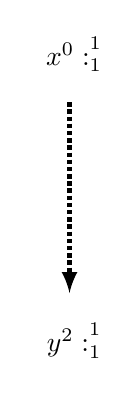
\begin{tikzpicture}[scale=\textwidth/20cm,samples=200]
          \draw[] (0, 8) circle (0pt) node{{ ${x^0 :}_{1}^{1}$}};
          % \draw[] (0, 7) circle (0pt) node{{ $1 : 1$}};
          % \draw[] (-3, 3) circle (0pt) node{\textbf{$2 : 1$}};
          % \draw[] (3, 3) circle (0pt) node{{ $3 : 1$}};
          \draw[] (0, 2) circle (0pt) node {{ ${y^2 :}_{1}^{1}$}};
        %
        % Control Flow Edges:
        \draw[  ultra thick, -latex, densely dotted,] (0, 7)  -- (0, 3);
        % \draw[  -latex] (0, 6.5)  -- node [left] {$x > 2 $}(-3, 3.5);
        % \draw[  -latex] (0, 6.5)  -- node [right] {$x \leq 2 $}(3, 3.5);
        % \draw[  -latex] (-3, 2.5)  -- node [left] {$y' \leq Q_m$}(0, - 0.5);
        % \draw[  -latex] (3, 2.5)  -- node [right] {$\top$}(0, - 0.5);
            \end{tikzpicture}
        \caption{}
          \end{centering}
          \end{subfigure}
      \caption{(a) The $\kw{ifQuery}$ program.
      (b) The abstract transition graph for $\kw{ifQuery}$.  
      (c) The estimated dependency graph for $\kw{ifQuery}$.}
      \label{fig:abscfg_ifQuery}
    \end{figure}